%%% LaTeX Template: Article/Thesis/etc. with colored headings and special fonts
%%%
%%% Source: http://www.howtotex.com/
% vim: set spell spelllang=es syntax=tex :

\documentclass[12pt]{article}
\usepackage[T1]{fontenc}
\usepackage{styles/apuntes-estilo}
\usepackage{styles/egyptian}
\usepackage{fancyhdr,lastpage}
\usepackage{hyperref}
\usepackage[inline]{enumitem}

\def\maketitle{

\makeatletter{
    \color{blue} \centering \huge \sc
    \textbf{
        Examen final libre 2022\\
        \small \vspace*{-8pt} \color{black}
        Parte práctica
        \vspace*{8pt}
    }\\
    \par
}
\makeatother

\makeatletter
% vim: set spell spelllang=es syntax=tex :
 {\centering \small 
    Introducción a la computación\\
    Departamento de Ingeniería de Computadoras \\
    Facultad de Informática - Universidad Nacional del Comahue \\
    \vspace{20pt} }
\makeatother

\vspace{-2.5cm}
\mbox{\hspace{-1cm}\includegraphics[width=3cm,height=3cm]{logos/uncoma.pdf}\hspace{13cm}
    \includegraphics[width=2.9cm,height=2.9cm]{logos/fai.pdf}}



}

% Custom headers and footers
\fancyhf{} % clear all header and footer fields
\fancypagestyle{plain}{\fancyhf{}}
\pagestyle{fancy}
\lhead{\footnotesize Primer examen parcial}
\rhead{\footnotesize \thepage\ }

\def\ti#1#2{\texttt{#1} & #2 \\ }

\begin{document}

\thispagestyle{empty}
\maketitle
\setlength{\parindent}{1pt}

\begin{enumerate}

    \item ¿Cuál es la representación de $21_{12}$ en las siguientes bases?

        \begin{enumerate}

            \item Base 4.

            \item Base 2.

            \item Base 8.

        \end{enumerate}

    \item ¿Cuál es rango de representación del los  sistemas \emph{de complemento a
        dos}, \emph{signo magnitud} y \emph{sin signo} con 6 bytes?

    \item ¿Cual es la representación en \emph{punto fijo} y \emph{complemento
        a 2} de los siguientes números si se utilizan 5 bits para la parte
        entera y 3 para la parte fraccionaria? Indicar cual es el error de
        representación (la diferencia entre el valor original y el
        almacenado).

        \begin{enumerate}

            \item $15.3$

            \item $-15.3$

        \end{enumerate}

    \item ¿Cuál es la representación hexadecimal del número $15.75$ cuando es
        almacenado utilizando el sistema de \emph{Punto Flotante IEEE-754 de
        precisión simple (32 bits)}?

    \item ¿Cuál es la representación hexadecimal de la codificación
        en \emph{ASCII} la cadena ``\emph{Final Libre/22}''?

    \item Considerando la imagen que se muestra abajo, aplique el esquema de
        codificación de imágenes visto en la práctica. \textbf{No olvide
        incluir la cabecera}. Asuma que 00 = blanco, 11 = negro y 01 =
        celeste. Muestre el resultado final expresado en hexadecimal.

    
\includegraphics[width=0.50\textwidth]{img/img_2020_1tpo-r.pdf}

    \item Si se tiene una imagen con 1024 píxeles de ancho, 256 píxeles de
        alto, y una profundidad de color de 7 bits por pixel ¿Cuántos colores
        distintos puede tener la imagen?

    \item Dado el siguiente programa:

        \begin{verbatim}
     0          LD  MAX
     1          JZ  END
     2          SUB NUM
     3          ST OUT
     4          J   END
     5  END:    HLT
     6  NUM:    2
     7  MAX:    16
        \end{verbatim}

        \begin{enumerate}

            \item ¿Cuál es la salida del programa?

            \item Si se compila el programa ¿Cuál sera el contenido binario de
                las direcciones \textbf{1}, \textbf{2} y \textbf{4}?

        \end{enumerate}

    \item Dado el siguiente programa en binario:

        \begin{verbatim}
    00 01001000
    01 01111111
    02 01001001
    03 10101010
    04 01101001
    05 11100010
    06 11011010
    07 00100000
    08 00101010
    09 00000101
    10 00000001
        \end{verbatim}

        ¿Cuál es la salida del programa?

    \item Si se extendiera el \textbf{MCBE} para que utilice 7 bits para el
        código de operación y 9 bits para el operando:

        \begin{enumerate}

            \item ¿Cuántos códigos de operación distintos podría soportar?

            \item ¿Cuántas celdas de memoria podría soportar?

            \item ¿Cuál seria el nuevo rango de los saltos?

        \end{enumerate}

    \item Muestre una secuencia de comandos que permita crear la estructura de
        directorios mostrada en la figura \ref{directorios}. Asuma que el
        directorio raíz (“/”) ya existe.

    \item Si el usuario se encuentra posicionado en el directorio \emph{E} del
        árbol de directorios mostrado en la figura \ref{directorios}:

        \begin{enumerate}

            \item Indique una secuencia de comandos para mover el archivo
                \emph{M} a la carpeta \emph{G} utilizando solo rutas
                relativas.

            \item Indique una secuencia de comandos para mover el archivo
                \emph{I} a la carpeta \emph{C} utilizando solo rutas
                absolutas.

        \end{enumerate}

\end{enumerate}

\subsection*{ \large\textbf{Anexo:} }

\textbf{Códigos de operación}

\begin{verbatim}
    010     LD
    011     ST
    100     ADD
    101     SUB
    110     JMP
    111     JZ
    001     HLT
    000     NOP
\end{verbatim}

\textbf{Tabla \emph{ASCII}:}

\begin{verbatim}
Dec Hex    Dec Hex    Dec Hex  Dec Hex  Dec Hex  Dec Hex   Dec Hex   Dec Hex
  0 00 NUL  16 10 DLE  32 20    48 30 0  64 40 @  80 50 P   96 60 `  112 70 p
  1 01 SOH  17 11 DC1  33 21 !  49 31 1  65 41 A  81 51 Q   97 61 a  113 71 q
  2 02 STX  18 12 DC2  34 22 "  50 32 2  66 42 B  82 52 R   98 62 b  114 72 r
  3 03 ETX  19 13 DC3  35 23 #  51 33 3  67 43 C  83 53 S   99 63 c  115 73 s
  4 04 EOT  20 14 DC4  36 24 $  52 34 4  68 44 D  84 54 T  100 64 d  116 74 t
  5 05 ENQ  21 15 NAK  37 25 %  53 35 5  69 45 E  85 55 U  101 65 e  117 75 u
  6 06 ACK  22 16 SYN  38 26 &  54 36 6  70 46 F  86 56 V  102 66 f  118 76 v
  7 07 BEL  23 17 ETB  39 27 '  55 37 7  71 47 G  87 57 W  103 67 g  119 77 w
  8 08 BS   24 18 CAN  40 28 (  56 38 8  72 48 H  88 58 X  104 68 h  120 78 x
  9 09 HT   25 19 EM   41 29 )  57 39 9  73 49 I  89 59 Y  105 69 i  121 79 y
 10 0A LF   26 1A SUB  42 2A *  58 3A :  74 4A J  90 5A Z  106 6A j  122 7A z
 11 0B VT   27 1B ESC  43 2B +  59 3B ;  75 4B K  91 5B [  107 6B k  123 7B {
 12 0C FF   28 1C FS   44 2C ,  60 3C <  76 4C L  92 5C \  108 6C l  124 7C |
 13 0D CR   29 1D GS   45 2D -  61 3D =  77 4D M  93 5D ]  109 6D m  125 7D }
 14 0E SO   30 1E RS   46 2E .  62 3E >  78 4E N  94 5E ^  110 6E n  126 7E ~
 15 0F SI   31 1F US   47 2F /  63 3F ?  79 4F O  95 5F _  111 6F o  127 7F DEL
\end{verbatim}

\begin{figure}

    \centering

    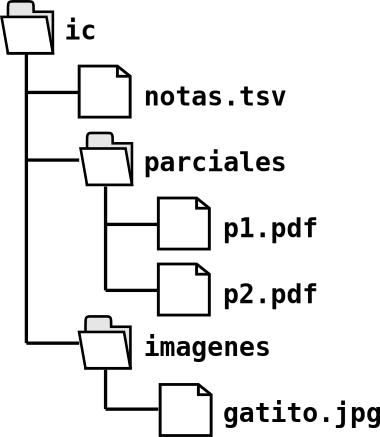
\includegraphics[width=0.5\textwidth]{img/directorios.pdf}

    \caption{Estructura de directorios I}

    \label{directorios}

\end{figure}

\end{document}
